%%%%%%%%%%%%%%%%%%%%%%%%%%%%%%%%%%%%%%%%%
% 
% Jalpaiguri Government Engineering College Survey Report Submission Format
% 
%%%%%%%%%%%%%%%%%%%%%%%%%%%%%%%%%%%%%%%%%
%\title{Title page with logo}
%----------------------------------------------------------------------------------------
%	PACKAGES AND OTHER DOCUMENT CONFIGURATIONS
%----------------------------------------------------------------------------------------

\documentclass[hidelinks,14pt]{extarticle}
\usepackage[english]{babel}
\usepackage[utf8x]{inputenc}
\usepackage{amsmath}
\usepackage{graphicx}
\usepackage[colorinlistoftodos]{todonotes}
\usepackage[cmintegrals,cmbraces]{newtxmath}
\usepackage{ebgaramond-maths}
\usepackage[T1]{fontenc}
\usepackage[hidelinks]{hyperref}
\usepackage[nottoc]{tocbibind}

\begin{document}
\begin{titlepage}

\newcommand{\HRule}{\rule{\linewidth}{0.5mm}} % Defines a new command for the horizontal lines

\center % Center everything on the page
 
 %----------------------------------------------------------------------------------------
%	LOGO SECTION
%----------------------------------------------------------------------------------------


\includegraphics[width=5cm]{fig/image.jpg}\\[0.3cm] % Include a department/university logo
 
%----------------------------------------------------------------------------------------

%----------------------------------------------------------------------------------------
%	HEADING SECTIONS
%----------------------------------------------------------------------------------------

\textsc{\LARGE Jalpaiguri Government Engineering \newline\newline College}\\[1cm] % Name of your university/college
\textsc{\Large Computer Science \& Engineering}\\[0.5cm] % Department Name
\textsc{\large \textbf{Survey Report}}\\[0.3cm] % SurveyReport 

%----------------------------------------------------------------------------------------
%	TITLE SECTION
%----------------------------------------------------------------------------------------

\HRule \\[0.3cm]
{ \huge \bfseries Project Title }\\[0.3cm] % Title of your document 
\HRule \\[1cm]

%For longer title comment the above 3 lines and use the lines below 
% \HRule \\[0.3cm]
% { \huge \bfseries Project Title \\ \large{As Never Seen Before in the History of Mankind}}\\[0.3cm] % Title of your document 
% \HRule \\[1cm]
 
%----------------------------------------------------------------------------------------
%	AUTHOR SECTION
%----------------------------------------------------------------------------------------

\begin{minipage}{0.4\textwidth}
\begin{flushleft} \large
\emph{Submitted by:}\\
John \textsc{Smith} \\% Your name
Roll: 14101104000 \\ % Your Roll No
Reg.: 14101011040000, 2014 % Registration Number and Year
\end{flushleft}
\end{minipage}
~
\begin{minipage}{0.4\textwidth}
\begin{flushright} \large
\emph{Project Supervisor:} \\
Dr. James \textsc{Smith}\\ % Supervisor's Name
\end{flushright}
\end{minipage}\\[1cm]



%----------------------------------------------------------------------------------------
%	DATE SECTION
%----------------------------------------------------------------------------------------

{\normalsize \today}\\ % Date, change the \today to a set date if you want to be precise


\vfill % Fill the rest of the page with whitespace

\end{titlepage}

\begin{abstract}
The abstract is a succinct, single-paragraph summary of your paper’s purpose, main points, method, findings, and conclusions, and is often recommended to be written after the rest of your report has been completed. The abstract\'s length should be minimum of 150 words and maximum of 250 words and should be confined within a paragraph. Use the active voice and past tense in the abstract, but present tense may be used to describe conclusion and implications.
\end{abstract}
\clearpage

\tableofcontents
\pagebreak

\section{Introductions}
\subsection{Topic Introduction}
\label{sec:1:1}
Give an overview of the subject area. By way of introduction, this reading section of the existing literature should take the form of an abstract of the general subject or study area and identify the discipline(s) within which it falls. From this analysis the problem or disorder you wish to research will emerge and constitutes the reason or condition which necessitates the research.

\subsection{Project Problem \& Aim}
\label{sec:1:2}
From the overview of the subject area follows the research problem, i.e. you have to identify the possible cause(s) of the disorder. This section states the problem that you are exploring. Next, you have to describe the research aim as it relates to solving the uncertainty or burning question you are interested in. It should explicitly hint towards the contribution you want to make with the intended study.

\section{Summary of Notation \& Theory}
\label{sec:2}
This section should provide a detailed description of the theory and concepts (mathematical or otherwise) related to the project. Use suitable use cases and diagrams as necessary.
For mathematical notations use the \LaTeX  \emph{equation} environment as shown in the code of this PDF.
Example equation:
\begin{equation}
\label{eq:1}
e^{\pi i} = -1
\end{equation}
For figures use the \emph{figure} environment. An example figure is shown in \autoref{fig:1}. Set the width of the figures to \emph{0.7 of linewidth} for consistency.
\begin{figure}[htbp]
\centerline{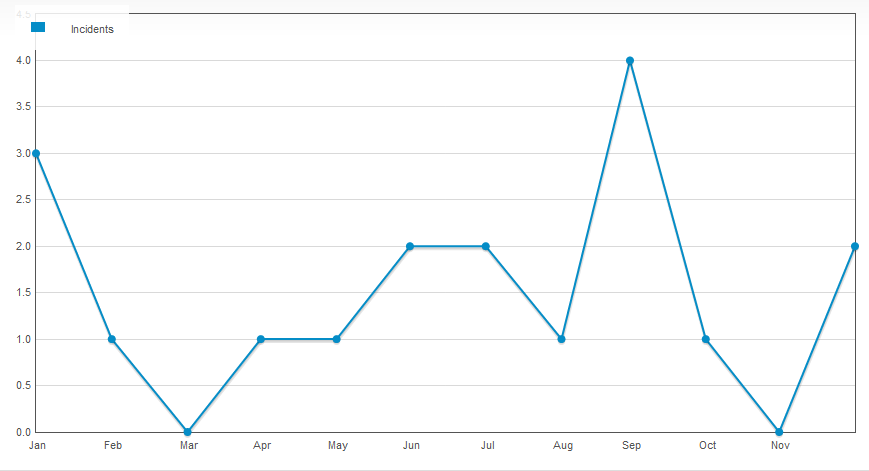
\includegraphics[width=0.7\linewidth]{fig/graph.png}}
\caption{Some Important Graph}
\label{fig:1}
\end{figure}

\section{Literature Review}
\label{sec:3}
In this section you should demonstrate that you are \textit{au fait} with the debates and issues raised in related literature. You should furnish a description of recent academic and empirical research in your chosen area. References to key texts and recently published articles should be made to convince that you appreciate their integrative relevance to your research area .

\section{Analysis of Related Works}
\label{sec:4}
Critical analysis of literature involves carefully examining the main ideas and relationships of an issue and providing a critique of existing literature. The critique is the critical evaluation of how well the literature represents the issue. Critical analysis often requires the author first to deconstruct a topic into its basic elements. These may include the history and origins of
the topic, its main concepts, the key relationships through which the concepts interact, research methods, applications of the topic, and so on. Figures and tables may be used to summarize and compare the various works and results thus drawing conclusion over the available approaches. A guide to using \emph{figures} has been demonstrated in \autoref{sec:2}.

Tables may be used as follows using the \emph{table} environment in \LaTeX as show in \autoref{tab:1}. In case you are dealing with a particularly large or fancy table, \emph{tabularx} package may be used.
\begin{table}
\centering
\caption{A Useful Table}
\label{tab:1}
\begin{tabular}{|c|c|c|c|c|c|}
\hline
Number of Values, $K$ & 16 & 8 & 4 & 2 & 1 \\ \hline
$log_2(K)$             & 4  & 3 & 2 & 1 & 0 \\ \hline
\end{tabular}
\end{table}
All tables \& figures must be labeled, and referred. Using \emph{hyperref} package can make life easier for you in this regard. 
All works referred in this report must be cited. For citing reference get the BibTeX list of the particular work. You may get the reference from \emph{Google Scholar} using the steps shown in \autoref{fig:2} and \autoref{fig:3}. Paste the BibTeX in \emph{biblist.bib} and refer the work \cite{lester1999writing}.
\begin{figure}[htbp]
\centerline{
\includegraphics[width=0.7\linewidth]{fig/Selection_028.png}}
\caption{Click on the Quotation Signs}
\label{fig:2}
\end{figure}

\begin{figure}[htbp]
\centerline{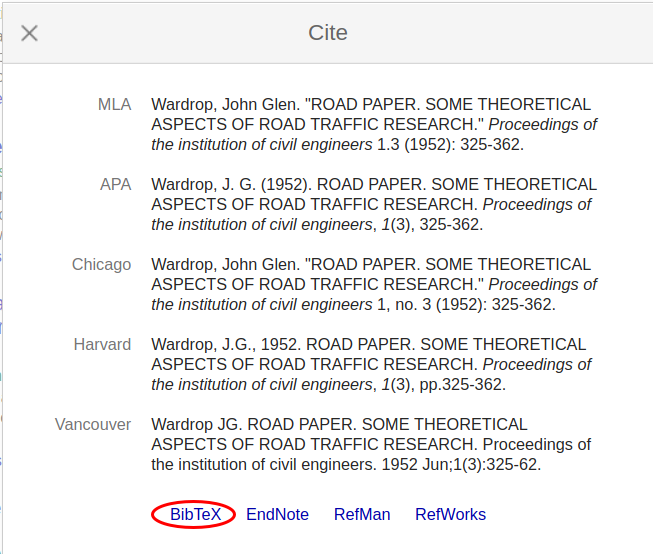
\includegraphics[width=0.7\linewidth]{fig/Selection_029.png}}
\caption{Click on BibTeX Link}
\label{fig:3}
\end{figure}


\section{Conclusion}
\label{sec:5}
In the first part of the conclusion, you should spend a brief amount of time summarizing what you’ve covered in your survey. This reiteration should not merely be a restatement of your problem statement or a collection of your topic sentences but should be a condensed version of your argument, topic, and/or purpose. 

TL;DR: This section should summarize your survey work keeping in ming the applications and future expansion of your work.



\newpage
\bibliographystyle{plain}
\bibliography{biblist}

\end{document}
